
%En primer lugar para describir el diseño de la aplicación se describirán los requisitos del sistema
%necesarios para la ejecución de la aplicación, posteriormente comentaremos que herramientas se va usar a lo largo
%del desarrollo.

\paragraph{}
Al igual que en el apartado referente al análisis del sistema, en el diseño de este también usaremos una metodología orientada
a objetos mediante UML.

\paragraph{}
Este proceso es mucho mas sencillo una vez que ya se ha especificado que hace el sistema en el capítulo anterior. También decir, que
al igual que el análisis del sistema, el diseño no contempla muchos detalles del sistema final, sólo una idea orientativa de como
se implementará el sistema.

\paragraph{}
En este capítulo no se han añadido descripciones de las clases que componen el sistema, para ello se encuentra disponible toda la
documentación del código, donde esta toda la información necesaria referente a las clases y archivos que componen la aplicación.

\section{Interfaz gráfica}

\paragraph{}
Tras los resultado que se han obtenido en la fase de analisis del sistema, es necesario desarrolar una interfaz sencilla y agradable
para el usuario de la misma. En el diseño de estos, se intentará en todo momento que el usuario no tenga la posibilidad de insertar
datos erroneos que lleven a una ejecución anómala de la aplicación.

\begin{figure}[H]
  \label{interfaz}
  \begin{center}
    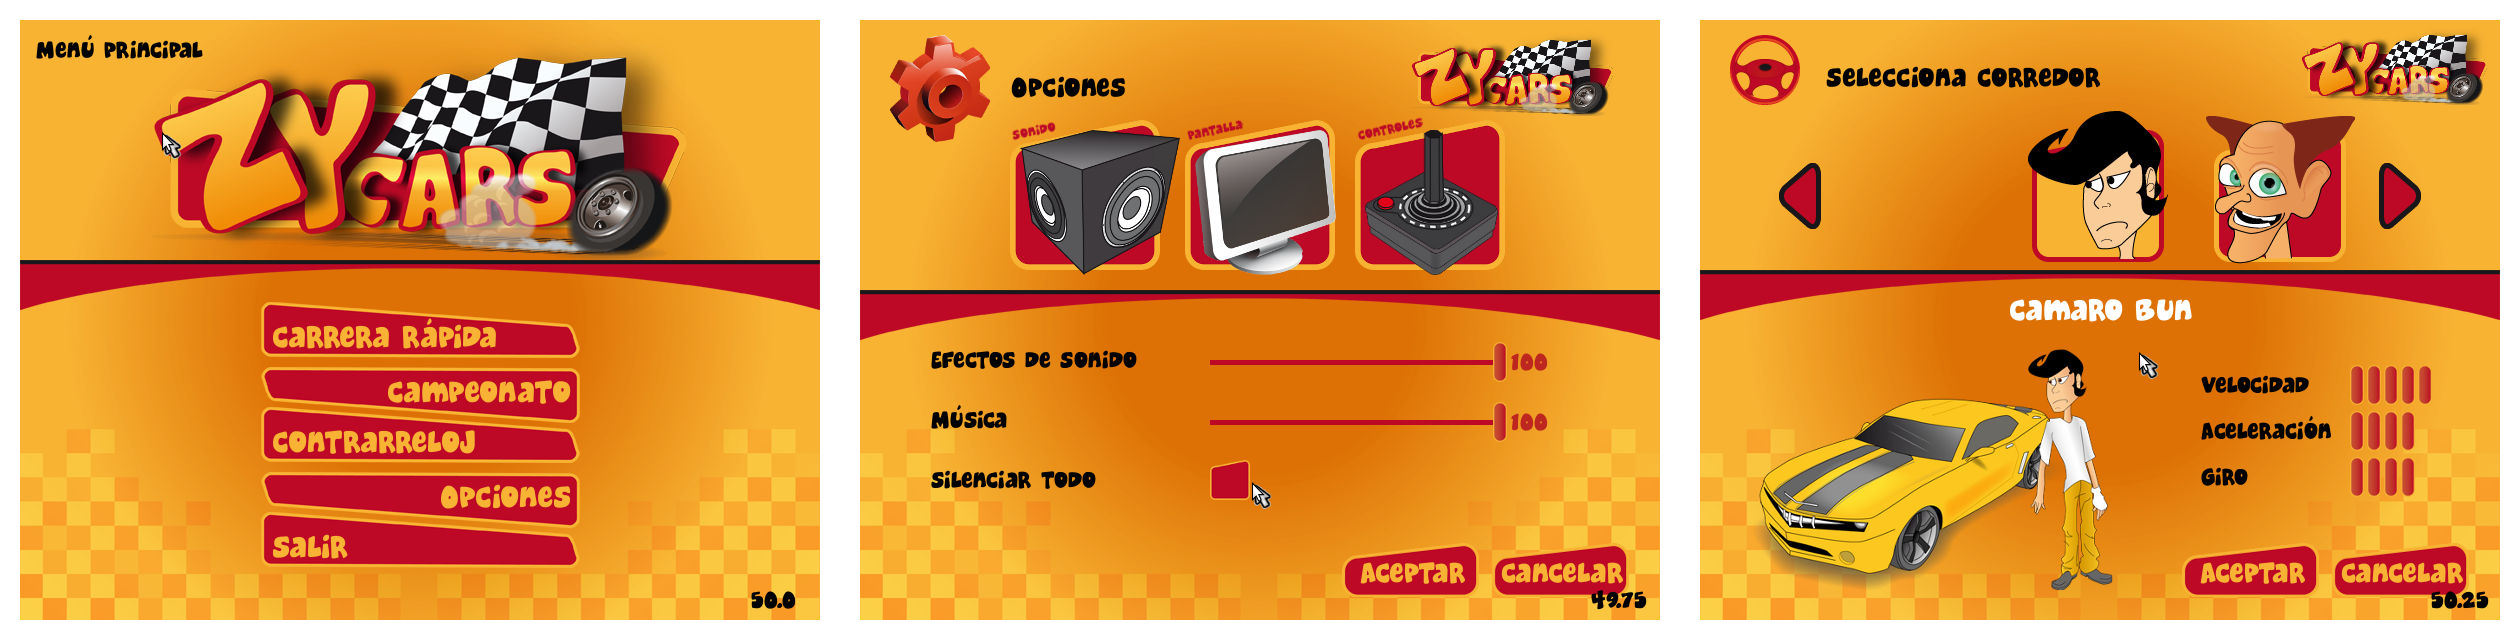
\includegraphics[scale=0.18]{imagenes/capturas/interfaz.png}
  \end{center}
  \caption{Diseño: Capturas de la interfaz del sistema}
\end{figure}

\subsection{Diagrama de interacción entre interfaces}

\paragraph{}
En la imagen que se muestra a continuación podemos observar la interacción entre las distintas interfaces graficas que se han 
desarrollado para la aplicación.

\begin{figure}[H]
  \label{diagrama_interaccion}
  \begin{center}
    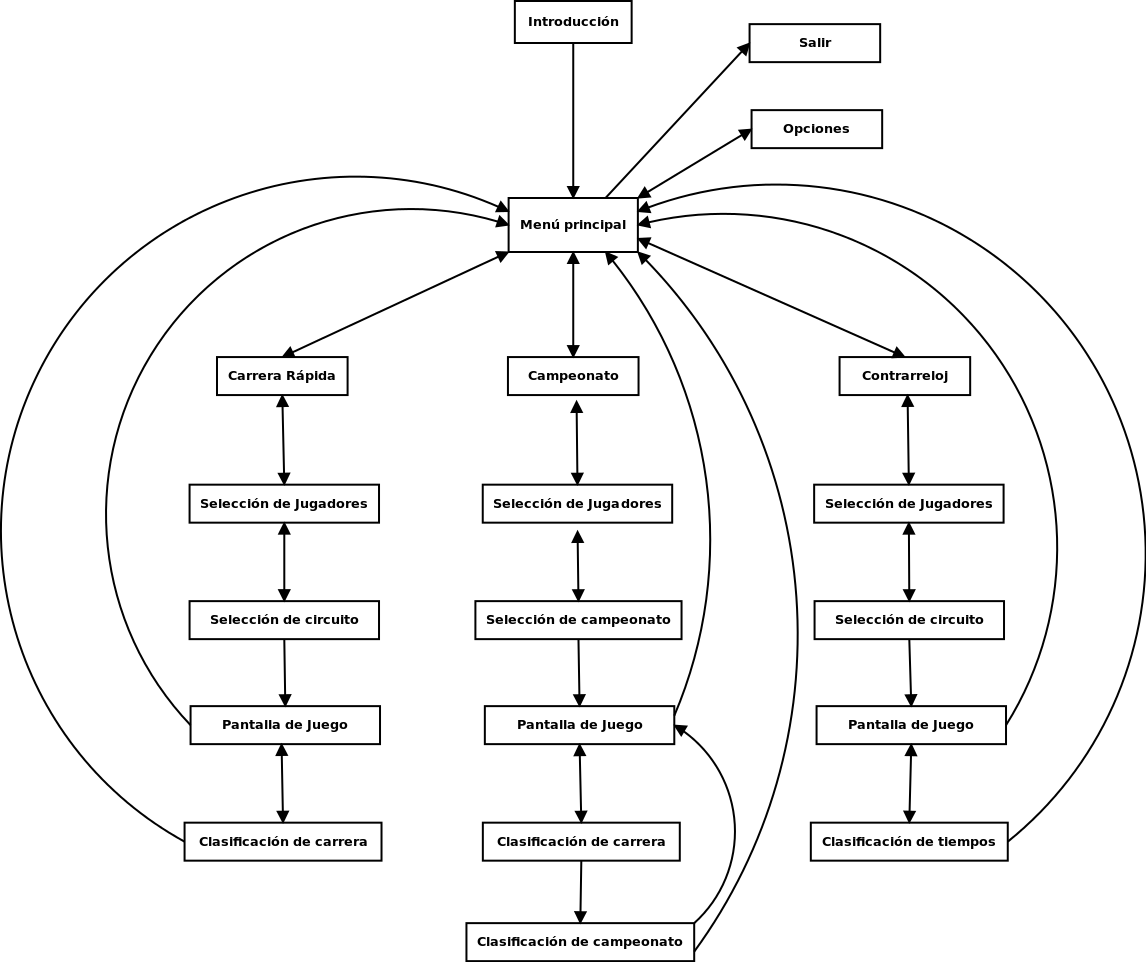
\includegraphics[scale=0.4]{imagenes/diseno/diagrama_interaccion.png}
  \end{center}
  \caption{Diseño: Diagrama de interacción}
\end{figure}

\section{Diagrama de clases de diseño}

A continuación se presenta el diagrama de clases de diseño de \emph{Zycars}.

\newpage

\begin{figure}[H]
  \label{diagrama_clases_diseno}
  \begin{center}
    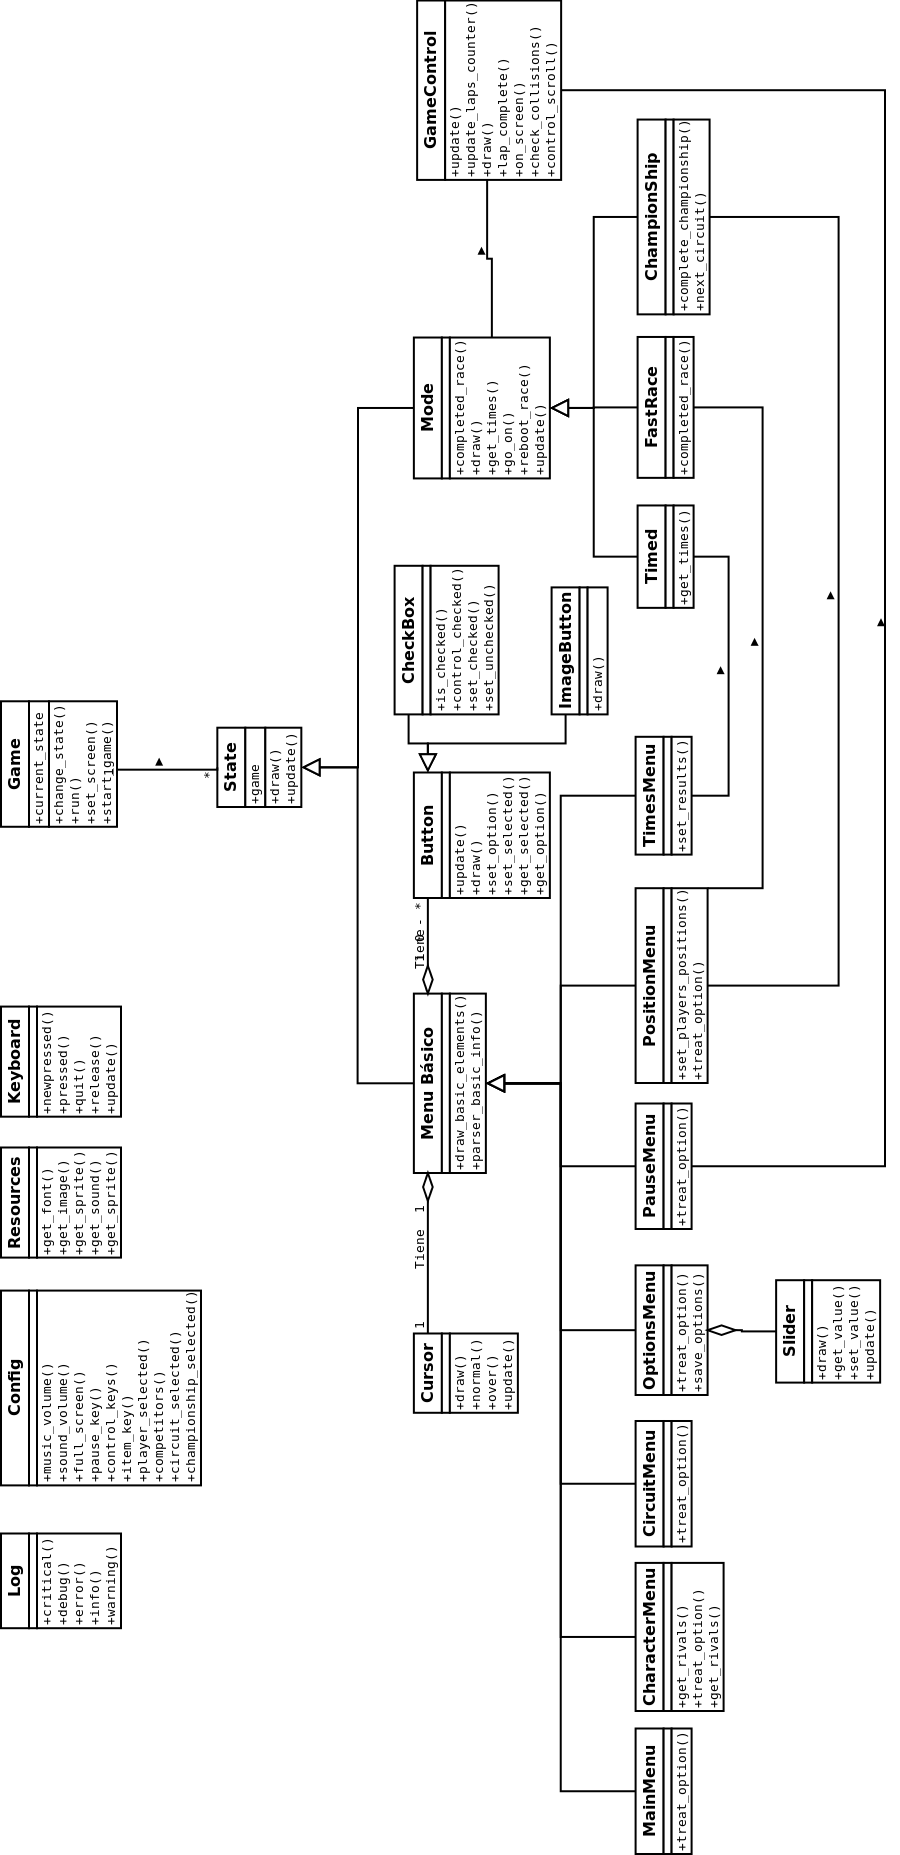
\includegraphics[scale=0.38]{imagenes/diseno/diagrama_clases_diseno1.png}
  \end{center}
  \caption{Diseño: Diagrama de clases de diseño 1}
\end{figure}

\begin{figure}[H]
  \label{diagrama_clases_diseno}
  \begin{center}
    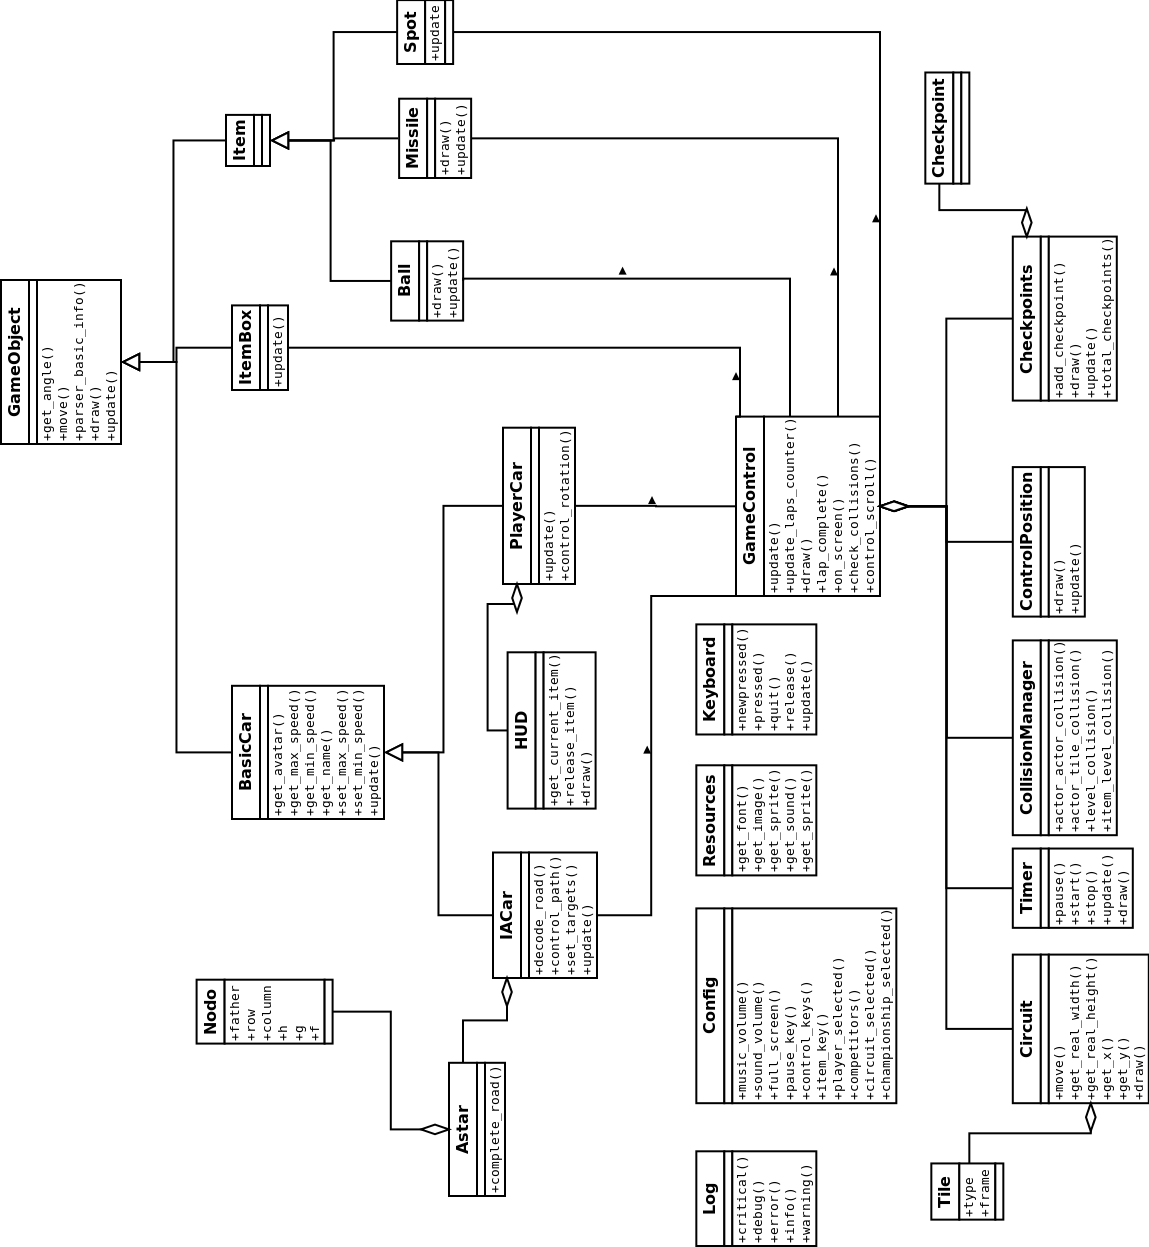
\includegraphics[scale=0.45]{imagenes/diseno/diagrama_clases_diseno2.png}
  \end{center}
  \caption{Diseño: Diagrama de clases de diseño 2}
\end{figure}

\section{Diagramas de secuencia}
lalalal
